\chapter{Features used to detect barcodes}
\label{sec:Features used to detect barcodes}

\section{Standard deviation}
\label{sec:Standard deviation}
One good method to exclude tiles that don't contain any code is to compute the standard deviation of each tile. Tiles which contain code will have a high standard deviation; hence all data with standard deviation under a certain threshold can be discarded. This fast method to reduce the amount of data before applying other more complicated features. 

\section{Structure tensor}
\label{sec:Structure tensor}
The structure tensor is an effective way to detect 1D-codes and to distinguish between 1D- and 2D-codes. The structure tensor for a tile is produced by first computing the gradients, this can be done by convolving the tile with a sobel filter. The structure tensor is then calculated in the following way:
\begin{center}
\begin{math}
	T = \begin{pmatrix}
			(I_{x})^2 & I_{x}I_{y} \\ I_{x}I_{y} & (I_{y})^2
		\end{pmatrix}
\end{math}
\end{center}
The structure tensor can be used in several ways to estimate the structure inside the tile. Areas that contain 1D-codes will have a one dimensional structure, i.e. the gradient in this area will only vary in one direction. On the other hand, areas that contain 2D-codes the variation will be fairly equal in both directions. The amount of variation of the gradient is measured by studying the eigenvalues of the structure tensor. The following feature is calculated for each tile:
\begin{center}
\begin{math}
f = \frac{(\lambda_1 - \lambda_2)^2}{\lambda_1^2+\lambda_2^2}
\end{math}
\end{center}
This feature is a measure of how likely the tile contains 1D-codes.

\section{FAST corner detection}
\label{sec:FAST corner detection}
FAST (Features from Accelerated Segment Test) is described in \citep{Rosten:2006} and \citep{Rosten:2005}. This is a method to detect corners in images, which is a good way to distinguish between 1D- and 2D-codes. For a pixel \textit{p} with intensity \textit{I}, consider a circle of 16 pixel and a threshold \textit{t}. The pixel is considered to be a corner if there exist a set of n contiguous pixels in the circle which are all brighter than \textit{I+t} or darker than \textit{I-t}. The algorithm is described in \ref{FAST}.

\begin{figure}[H]
\centering
	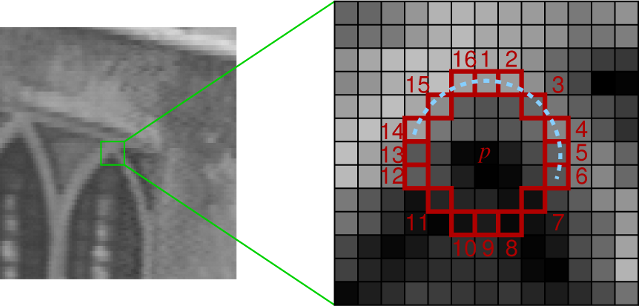
\includegraphics[scale=0.5]{FAST}
	\caption{Image describing FAST corner detection}
	\label{FAST}
\end{figure}

\section{Distance map}
\label{sec:Distance map}
A method for barcode detections using a distance map is described in \citep{Bodnar}. The objective of this method is to first calculate the edges in the image by using the canny edge detection algorithm. After that a distance transform is used which in each pixel calculates the closest distance to an edge. There after the mean and standard deviation for the distance map are calculated which are then used as features. The distance map has in this system been used only for detection of 1D-codes.
 
\section{Local binary pattern}
\label{sec:Local binary pattern}
Local binary pattern, which is described in \citep{Pietikainen:2010}, is a method that can be used for detection of 2D-codes. The basic idea is to compute a binary code for every pixel, based on the difference of the intensity between the pixel and the surrounding pixels, illustrated in \ref{LBP}. The binary code will then be transformed to a decimal scalar value. If a 3x3 neighborhood is used there will be 256 different possible values. For each block a histogram will be calculated for all these values. Every bin in the histogram will then be used as a feature. If there is a bin for every possible value, there will be 256 features.

\begin{figure}[H]
\centering
	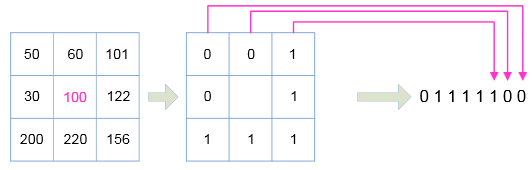
\includegraphics[scale=0.5]{LBP}
	\caption{Image describing local binary pattern}
	\label{LBP}
\end{figure}

% Local Variables:
% TeX-master: "main.tex"
% End:
